\documentclass[
    11pt,
    a4paper,
    egregdoesnotlikesansseriftitles,
    toc=chapterentrywithdots,
    openany,
    oneside,
    titlepage,
    parskip=half,
    headings=normal,  % reduces heading size
    listof=totoc,
    bibliography=totoc,
    index=totoc,
    captions=tableheading,  % caption below table
    chapterprefix,
    listof=flat,
    final
]{scrbook}


% details about your thesis
\newcommand{\titel}{Entwicklung eines modularen Synthesizers}
\newcommand{\artderarbeit}{Projektarbeit}  % {Bachelorarbeit,Masterarbeit}
\newcommand{\autor}{Altaher Ahmad, Balbach Thomas, Dilman Viktor, Kirschner Christoph, Sedlmeier Toni }
\newcommand{\studiengang}{MSY}  % {Informatik,Wirtschaftsinformatik,Medieninformatik}
\newcommand{\ausgabe}{18.10.2022}
\newcommand{\abgabe}{--}
\newcommand{\erstgutachter}{Prof. Dr.Alexander von Hoffmann}
\newcommand{\logo}{figures/TH-Nuernberg-RGB.png}
\newcommand{\keywords}{hot, fuzz}
 

% custom head and foot
\usepackage[automark]{scrlayer-scrpage}
\pagestyle{scrheadings}
\ihead{\headmark}
\chead{}
\ohead{\pagemark}
\renewcommand*\chaptermarkformat{\chapappifchapterprefix{\ }% 
  \thechapter.\enskip}

\usepackage{titlesec}


\RedeclareSectionCommand[tocindent=0pt]{section}
\RedeclareSectionCommand[tocindent=0pt]{subsection}
\RedeclareSectionCommand[tocnumwidth=30pt, beforeskip = -30pt]{chapter}


\usepackage{scrhack}

% other packages
\usepackage[utf8]{inputenc}
\usepackage[T1]{fontenc}
\usepackage{lmodern,relsize,textcomp,csquotes}
\usepackage{amsmath,amsfonts}
\usepackage[ngerman,ngerman]{babel}  % flip for German thesis
\usepackage[final]{graphicx}
\usepackage{setspace,geometry,xcolor}
\usepackage{makeidx}
\usepackage{paralist,ifthen,todonotes}
\usepackage{url}
%\usepackage[toc]{glossaries}
\usepackage{pdfpages}
\usepackage[style = numeric, backend = bibtex]{biblatex}


% table setup
\usepackage{longtable}
\usepackage{array}
\usepackage{ragged2e}
\usepackage{lscape}

% pdf hyperref
\usepackage[
    bookmarks=true,
    bookmarksopen=true,
    bookmarksnumbered=true,
    bookmarksopenlevel=1,
    pdftitle={\titel},
    pdfauthor={\autor},
    pdfcreator={\autor},
    pdfsubject={\titel},
    pdfkeywords={\keywords},
    pdfpagelabels=true,
    colorlinks=true,
    linkcolor=red,
    urlcolor=magenta,
    citecolor=cyan,
    filecolor=magenta,
    menucolor=red,
    plainpages=false,
    hypertexnames=true,
    linktocpage=true,
]{hyperref}


% configure your listings style
\usepackage{listings}
\lstset{
	tabsize=3,
	extendedchars=true,
	frame=single,
	showstringspaces=true,
	numbers=left,
	numberstyle=\small,
	breakautoindent=true,
	basicstyle=\small
}

\renewcommand{\lstlistingname}{Auflistung} % Aendert Listing zu Auflistung
\renewcommand{\lstlistlistingname}{Auflistungsverzeichnis} % Aendert Listing zu Auflistung

% page setup
% \setlength{\topskip}{\ht\strutbox}
\geometry{paper=a4paper,left=3cm,top=2cm,right=2cm,bottom=2cm}
\onehalfspacing
\frenchspacing
\clubpenalty = 10000
\widowpenalty = 10000 
\displaywidowpenalty = 10000

% some commands
\newcommand{\ua}{\mbox{u.\,a.\ }}
\newcommand{\zB}{\mbox{z.\,B.\ }}
\newcommand{\dahe}{\mbox{d.\,h.,\ }}
\newcommand{\bzw}{\mbox{bzw.\ }}
\newcommand{\bzgl}{\mbox{bzgl.\ }}
\newcommand{\eg}{\mbox{e.\,g.\ }}
\newcommand{\ie}{\mbox{i.\,e.\ }}
\newcommand{\wrt}{\mbox{w.\,r.\,t.\ }}
\newcommand{\etal}{\mbox{\emph{et.\,al.\ }}}

% load glossary entries
%\makenoidxglossaries
%\loadglsentries{glossary}

%\bibliographystyle{ieeetran}
\bibliography{refs_new}
\nocite{*}

\begin{document}

\setcounter{secnumdepth}{3}  % numerate subsections
\setcounter{tocdepth}{2}  % ...but don't include them in toc

\frontmatter
\thispagestyle{empty}
\pdfbookmark[1]{Cover}{cov}
\begin{titlepage}

\begin{center}


\includegraphics[width=\linewidth]{figures/TH-Nuernberg-RGB.png}\\[1cm]
\LARGE{Fakultät Elektrotechnik Feinwerktechnik Informationstechnik}\\[2cm]

\huge
\textbf{\titel}\\[1cm]
%
\Large
\artderarbeit~im \studiengang\\[1cm]
%
\large
vorgelegt von

\Large
\autor\\[0.5cm]
\small

\vspace*{\fill}

\large
\begin{tabular}{p{3cm}p{8cm}}\\
%Ausgabe:  & \quad \ausgabe\\[1.2ex]
Abgabe: & \quad \abgabe\\[1.2ex]
Prüfer:  & \quad \erstgutachter\\[1.2ex]
%discomment "Betreuer" and "Unternehmen" for a thesis in a company
%Betreuer: & \quad \betreuer\\
%Unternehmen: & \quad \unternehmen
\end{tabular}
\end{center}

\begin{center}
\copyright\,\the\year
\end{center}

\vspace{-0.5cm}
\singlespacing
\small

\end{titlepage}
\cleardoublepage

% download the following form and complete it (hit save in your editor)
% https://intern.ohmportal.de/fileadmin/Gelenkte_Doks/Abt/SZS/SB/%SB_0050_FO_Pruefungsrechtliche_Erklaerung_und_Erklaerung_zur_Veroeffentlichung_der_Abschlussarbeit_public.pdf

\includepdf{pruefungsrechtliche_erklaerung.pdf}\cleardoublepage

%\thispagestyle{empty}
\section*{Kurzdarstellung}
\label{sec:kurzdarstellung}
Kurze Zusammenfassung der Arbeit, höchstens halbe Seite.
Deutsche Fassung auch nötig, wenn die Arbeit auf Englisch angefertigt wird.

\blindtext


\section*{Abstract}
\label{sec:abstract}
\emph{Only if thesis is written in English.}

\blindtext
\cleardoublepage

%\titleformat{\chapter}
%  {\Large\bfseries} % format
%  {}                % label
%  {0pt}             % sep
%  {\huge}           % before-code
%  
\tableofcontents\cleardoublepage

\mainmatter
\chapter{Einleitung}
\label{ch:intro}

\chapter{Konzepte}
\label{ch:concept}

\section{Zielsetzung}
\label{sec:zielsetzung}
Wie bereits in Kapitel \ref{ch:intro} beschrieben, dient diese Projektarbeit zur Wissenserweiterung im Bereich der analogen Schaltungstechnik.
Darüber hinaus soll im Zuge dieser Arbeit ein einsetzbarer modularer Synthesizer gebaut werden, der zu elektronischen Klangerzeugung genutzt werden kann. 
Der Synthesizer soll aus verschiedenen Modulen bestehen, welche unabhängig von einander genutzt werden können. 
Der weitere Aufbau wird in Abschnitt \ref{sec:AufbauSynth} genauer beschrieben. 
Darüber hinaus werden in Abschnitt \ref{sec:AnalogePrinzipien} grundlegende Prinzipien erläutert, die insbesondere bei der elektronischen Klangerzeugung Anwendung finden.


\section{Aufbau eines modularen Synthesizers}
\label{sec:AufbauSynth}
Wie bereits in Abschnitt \ref{sec:zielsetzung} erläutert, besteht ein modularer Synthesizer aus mehreren vereinzelten Modulen. 
Diese Module können mit Kabeln verbunden und somit in Interaktion miteinander gebracht werden. 

Um eine grundlegende Funktion zu ermöglichen, ist ein Basisumfang an Modulen nötig.
Die hierfür nötigen Komponenten oder Module werden im Folgenden aufgelistet und kurz erläutert.

\begin{itemize}
	\item Netzteil:\newline
	Das Netzteil ist elementarer Bestandteil des Synthesizers und stellt die benötigten Spannungslevel zur Versorgung der einzelnen Module bereit.
	Insbesondere für den Einsatz von Operationsverstärkern ist es nötig symmetrische Spannungsversorgungen bereit zu stellen.
	
	\item LFO: \newline
	Ein LFO ("Low Frequency Oscillator") wird genutzt, um niederfrequente Signale zu erzeugen.
	Typischerweise wird dieses Modul genutzt, um andere Module anzusteuern.
	
	\item VCO: \newline
	Der VCO ist ein spannungsgesteuerter Oszillator und stellt die Basis bei analogen Synthesizern dar.
	Über eine Steuerspannung kann die Frequenz des erzeugten Signals und somit die Tonhöhe verändert werden. 
	Verbreitete Signale zur elektronischen Tonerzeugung stellen das Sägezahn- und das Rechtecksignal dar.
	
	\item Sequenzer: \newline
	Der Sequenzer erzeugt seriell alternierende Spannungsfolgen, die durch verschiedene Kippschalter und Potentiometer sowohl die einzelnen Spannungspegel als auch die gesamte Geschwindigkeit des Signals variieren. In der Regel werden die Ausgangssignale des Sequenzers zur Ansteuerung weiterer Module – den sogenannten Spannungsgesteuerten-Modulen – hergenommen. Neben den Oszillatoren bildet der Sequenzer somit die Basis der Synthesizer-Module.
	\item Filter
	\item Mischer
	\item Gehäuse : \newline
	Um den Synthesizer gut bedienen zu können und um die enthaltenen Komponenten vor schädlichen Einflüssen zu Schützen ist es sinnvoll, 
	die Module in einem Gehäuse zu verbauen. Dieses besteht üblicherweise aus zwei Schienen mit Anschraubmöglichkeiten, 
	auf welchen die Frontplatten der einzelnen Module geschraubt werden können.  
\end{itemize}

Um den groben Aufbau und die dahinter liegende Struktur zu verdeutlichen, ist in Abbildung xxx die grobe Produktarchitektur aufgezeigt.


\begin{figure}[h]
	\centering
	\setlength{\fboxsep}{1pt} %Abstand der Linien zur Abbildung
	\setlength{\fboxrule}{1pt} %Dicke der Linie
	\fbox{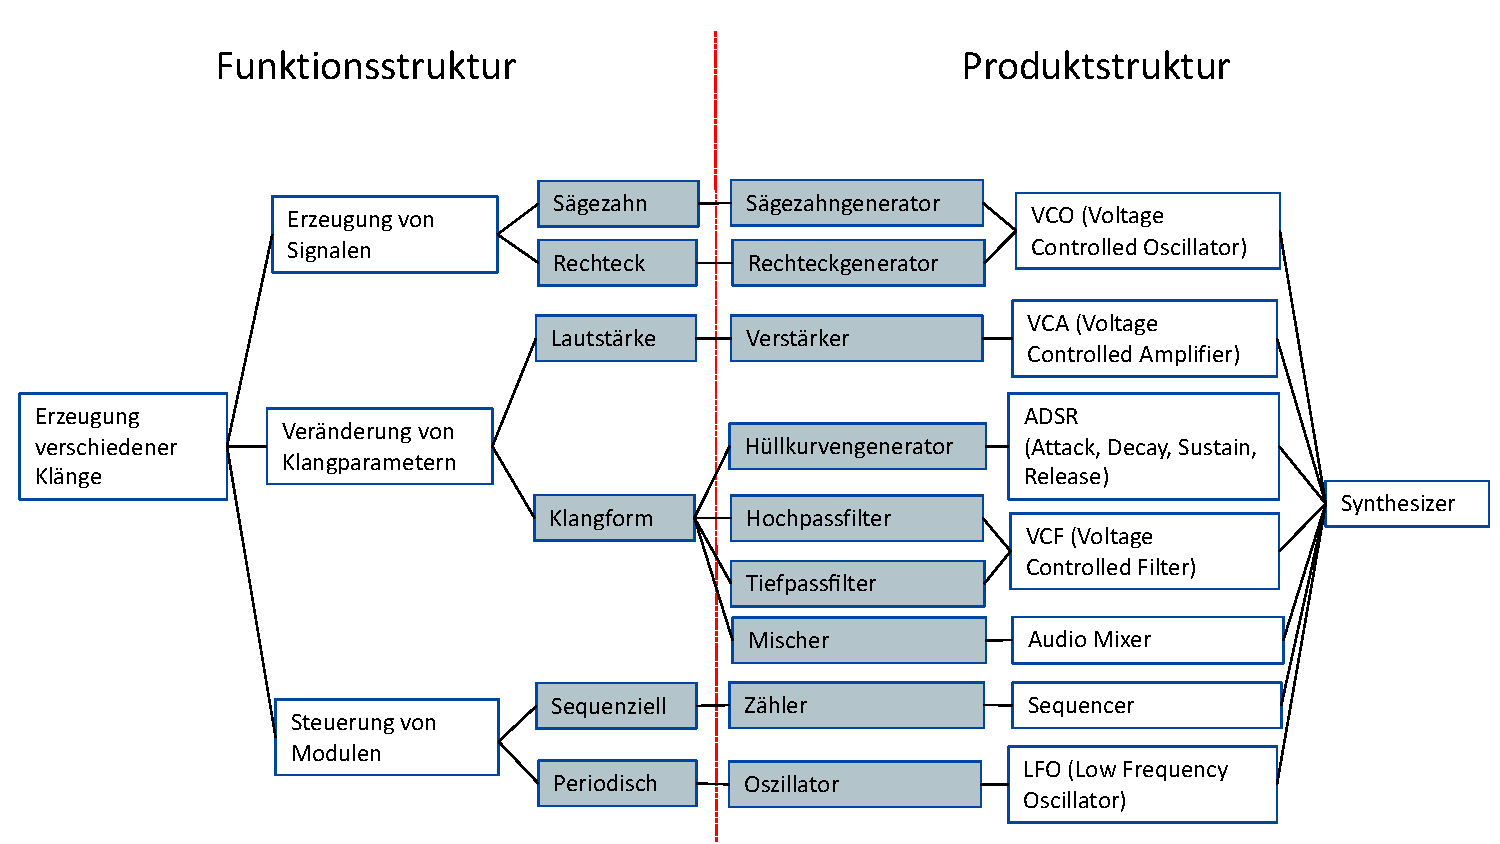
\includegraphics[width=0.8\textwidth]{figures/Produktarchitektur.pdf}}
	\caption{Produktarchitektur des modularen Synthesizers}
	\label{fig:fig:Produktarchitektur}
\end{figure}


\newpage
\section{Grundlegende analoge Prinzipien}
\label{sec:AnalogePrinzipien}






\chapter{Netzteil}
\label{ch:Netzteil}

\section{Allgemeines}
Um eine fehlerfreie Funktion aller weiteren Module zu gewährleisten, ist es wichtig, dass eine geeignete Spannungsversorgung bereitgestellt wird. 
Insbesondere für die Opamp-Schaltungen ist es wichtig, dass eine störfreie symmetrische Spannung bereitgestellt wird. 
Im Bereich der modularen Synthesizer wird hier typischerweise eine Spannung von +/- 12 V benötigt. Diese Spannungspegel werden durch eine geignete Beschaltung von Dioden und Kondensatoren generiert, welche in Abschnitt \ref{sec:netzteil_schaltplan} bzw. \ref{sec:netzteil_umsetzung} genauer erläutert wird. Hierbei wird die für modulare Synthesizer typischerweise eingesetzte Wannenstecker-Belegung verwendet. Diese wird entsprechend in allen Modulen eingesetzt!


\section{Schaltplan}
\label{sec:netzteil_schaltplan}
bla bla bla

\section{Umsetzung}
\label{sec:netzteil_umsetzung}
bla bla bla
\chapter{LFO}
\label{ch:concept}

\section{Allgemeines}
Wie bereits in Kapitel \label{ch:concept} beschrieben, wird der LFO genutzt, um niederfrequente Signale zu erzeugen. 
Diese Signale werden typischerweise zur Steuerung von nachgelagerten Modulen, wie etwa dem LFO (siehe Kapitel \ref{ch:VCO}), verwendet.
Hierdurch kann beispielsweise die Frequenz des VCO angepasst werden. 
Neben der Frequenz, die der LFO ausgibt, ist auch die entsprechende Signalform für den Klang entscheidend. Hier sind beispielsweise Signalformen, wie Dreieck oder Rechteck möglich.

\section{Schaltplan}
Im Folgenden wird näher auf den Schaltplan des LFO eingegangen, welcher in Abbildung xx zu sehen ist. 
Ein Bauteil von zentraler Bedeutung ist hierbei der Vierfach-Operationsverstärker TL074P. In der gezeigten Schaltung wird dieser als Integrator, Schmitt Trigger, Buffer und LED-Treiber verwendet.
Die grundlegende Funktionsweise dieser Funktionsgruppen wurde bereits in Abschnitt \ref{sec:AnalogePrinzipien} erläutert und wird deshalb nicht erneut aufgezeigt.
 

\section{Platine}
bla bla bla

\section{Mechanischer Aufbau}
bla bla bla
\chapter{VCO}
\label{ch:VCO}
\section{Allgemeines}

VCO steht für \textit{Voltage Controlled Oscillator} und bezeichnet einen spannungsgesteuerten Oszillator.
Dieses Modul stellt die Basis aller analogen Synthesizers da. 
Mit einem spannungsgesteuerten Oszillator lassen sich verschiedene Signale generieren, deren Frequenz sich mit der angelegten Steuerspannung verändert.
Analoge Synthesizer orientieren sich oft am 1V/Oktave-Standard.
Dieser besagt, dass sich die Frequenz des Signals mit jedem Volt verdoppelt.
Dies ist von Vorteil, da das Verhältnis zwischen Musiknoten und deren zugeordneten Frequenzen ebenfalls exponentiell ist.
Die tiefste C-Note entspricht beispielsweise einer Frequenz von 16,35 Hz.
Wenn man eine Oktave nach oben geht, verdoppelt sich die Frequenz beim nächsten C auf etwa 32 Hz. Typische Signale bei analogen Synthesizern können der Abbildung \ref{fig:Waveforms} entnommen werden. \cite{MakeSynth}

\begin{figure}[h]
	\centering
	\setlength{\fboxsep}{1pt} %Abstand der Linien zur Abbildung
	\setlength{\fboxrule}{1pt} %Dicke der Linie
	\fbox{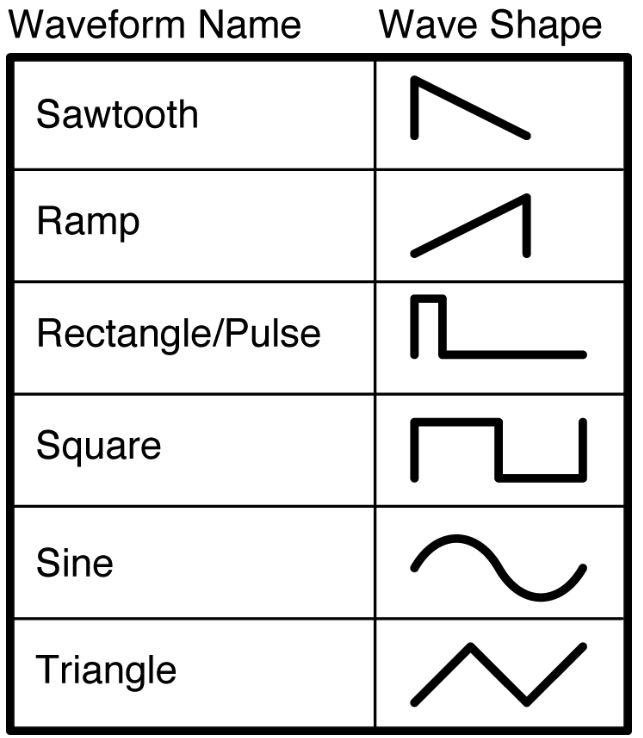
\includegraphics[width=0.5\textwidth]{figures/Waveforms}}
	\caption{Typische Signale bei analogen Synthesizern \cite{MakeSynth}}
	\label{fig:Waveforms}
\end{figure}

Bei dieser Umsetzung des VCOs wurde sich auf die Realisierung eines Sägezahn- und eines Rechtecksignals konzentriert, da diese aufgrund ihrem hohen Oberwellenanteil markant-hörbare Geräusche erzeugen.
Ein Sinussignal hingegen stellt einen harmonischen Verlauf dar, der sich ebenfalls im Klang äußert.
Hörbare Schwingungen werden mithilfe einer Oszillatorschaltung realisiert, auf die im Folgenden näher eingegangen wird.

\begin{figure}[h]
	\centering
	\setlength{\fboxsep}{1pt} %Abstand der Linien zur Abbildung
	\setlength{\fboxrule}{1pt} %Dicke der Linie
	\fbox{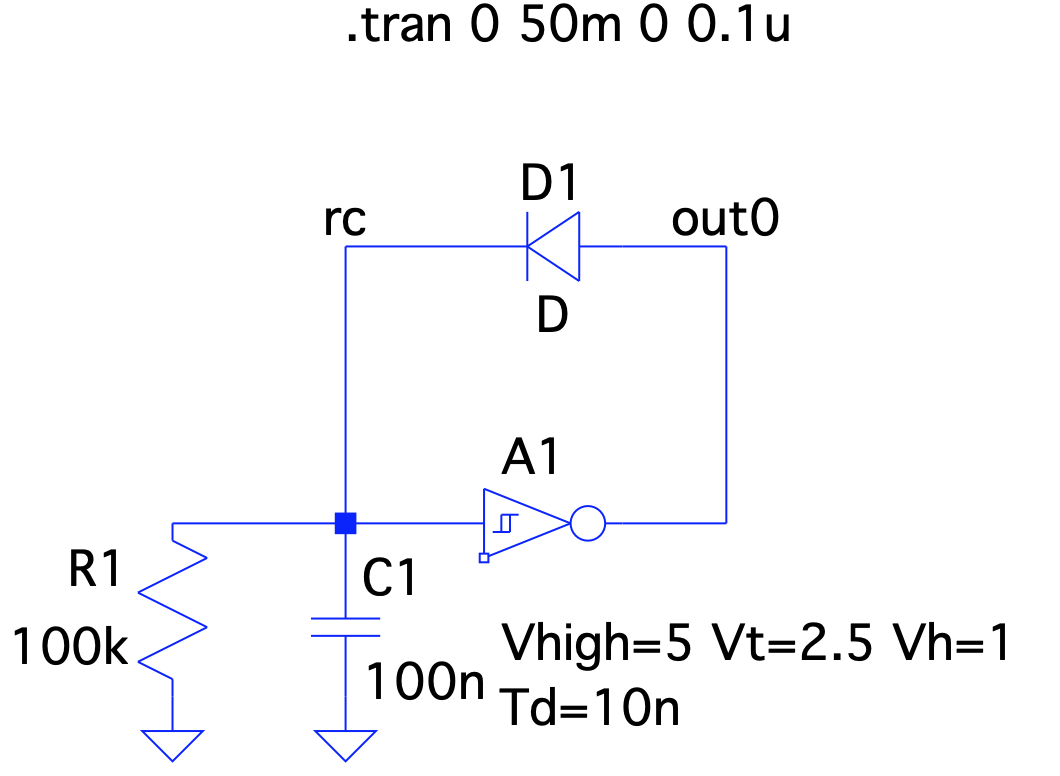
\includegraphics[width=0.8\textwidth]{figures/Oszillator_Schaltbild}}
	\caption{Oszillatorschaltung}
	\label{fig:Oszillatorschaltung}
\end{figure}

Um die Oszillatorschaltung (vgl. Abbildung \ref{fig:Oszillatorschaltung}), die den Kern des VCOs darstellt, zu verstehen, erfolgt die Betrachtung des Punktes \textit{rc}.
Zu Beginn liegt keine Spannung an, weil der Kondensator leer ist und noch kein Strom durch die Diode fließt. 
Das bedeutet, dass am Ausgang des Schmitt-Trigger-Inverters eine Spannung anliegt, da der Eingang unter dem unteren Eingangsschwellenwert liegt. 
Dadurch erfolgt ein Stromfluss vom Ausgang des Schmitt-Triggers über die Diode zu dem Punkt \textit{rc}. 
Da der Kondensator zunächst leer ist, fließt der ganze Strom in diesen hinein.
Während sich der Kondensator auflädt, steigt die Spannung an dem Punkt \textit{rc} rapide an.
Dieser Spannungsanstieg wird vom Schmitt-Trigger-Eingang registriert. 
Als Reaktion darauf fällt der Ausgang auf 0 V ab, sobald der Kondensator aufgeladen ist und die Spannung die obere Eingangsschwelle überschreitet.
Das bedeutet, dass kein zusätzlicher Strom durch die Diode fließt und sich der Kondensator wieder entlädt. 
Da der Widerstand die Strommenge begrenzt, die durchfließen kann, wird der Kondensator nicht sofort entladen. 
Auf dem Spannungsdiagramm entsteht also ein langsamer Abfall. 
Das geht so lange, bis der untere Schwellenwert des Schmitt-Trigger-Inverters erreicht wird. 
Sobald diese Schwelle auf dem Weg nach unten unterschritten ist, beginnt der Zyklus von neuem.
Die Simulation der Schaltung ergibt den Spannungsverlauf am Punkt \textit{rc} in Abbildung \ref{fig:Oszillator_Signalverlauf}.

\begin{figure}[h]
	\centering
	\setlength{\fboxsep}{1pt} %Abstand der Linien zur Abbildung
	\setlength{\fboxrule}{1pt} %Dicke der Linie
	\fbox{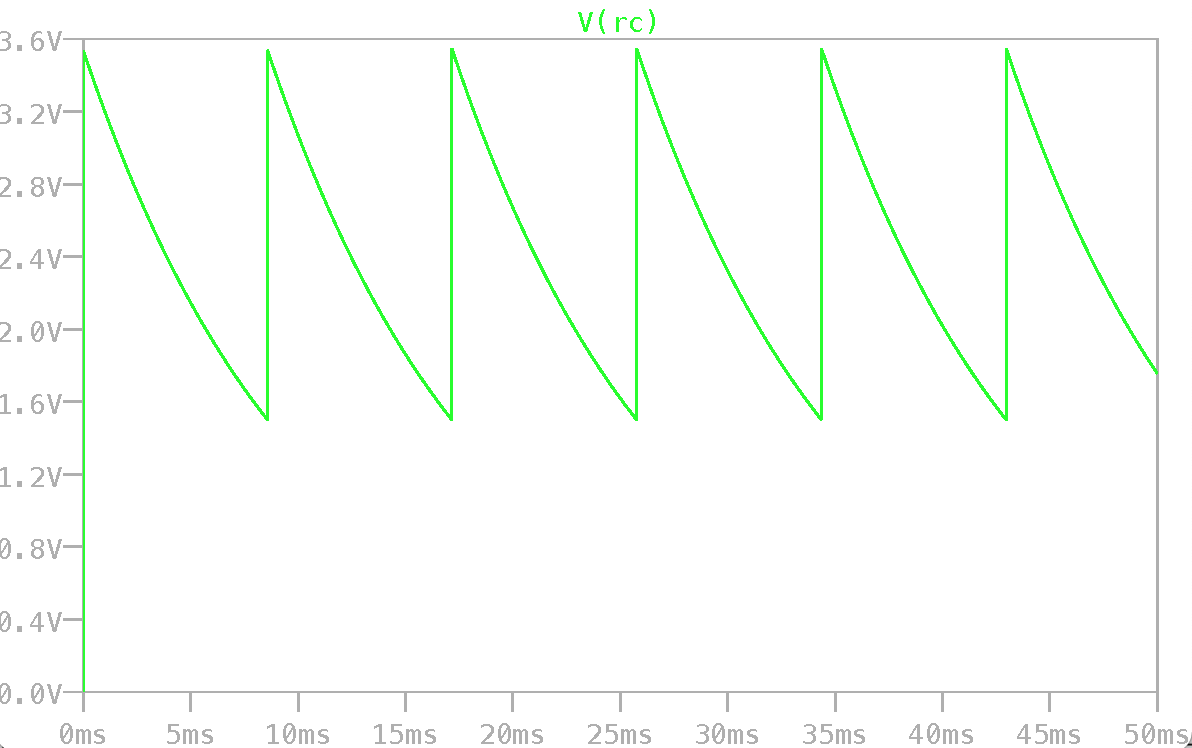
\includegraphics[width=0.8\textwidth]{figures/Oszillator_Signalverlauf}}
	\caption{Oszillator Signalverlauf}
	\label{fig:Oszillator_Signalverlauf}
\end{figure}

\newpage

Die Frequenz des entstandenen Sägezahnsignals hängt maßgeblich von dem Entladungsvorgang des Kondensators ab.
Die Geschwindigkeit dieses Entladungsvorganges wird widerum durch genau zwei Faktoren bestimmt: die Kapazität des Kondensators und der Wert des Widerstands.
Um den VCO an die Volt/Oktave-Norm anzupassen, muss die Beziehung zwischen Spannungseingang und Frequenzausgang ebenfalls exponentiell sein, da im Grunde genommen Spannungen auf Musiknoten abgebildet werden. 
Transistoren sind hier besonders geeignet, da das Verhältnis zwischen der an ihrer Basis angelegten Spannung und dem Strom, den sie zwischen Kollektor und Emitter fließen lassen, exponentiell ist.
Die Basisspannung kann mithilfe eines Potentiometers eingestellt werden.
Zu beachten ist allerdings, dass bei einem üblichen NPN-Transistor die Kollektor-Emitter Strecke ab etwa einer BasisSpannung von 600 -- 700 mV niederohmig wird und der Oszillator bei Anliegen dieser Schwellspannung nicht mehr schwingt. 
Liegt keine Spannung an, ist die Kollektor-Emitter Strecke hochohmig und der Oszillator kann ebenfalls nicht mehr schwingen.
Der durch Ausprobieren ermittelte nutzbare Spannungbereich beträgt etwa 350 -- 550 mV.
Dies wird mithilfe eines einstellbaren Spannungsteilers realisiert. 

Die verwendete Schaltung 
in Abbildung \ref{fig:VCO_Stromlaufplan} 
ist zu großen Teilen an ein \textit{DIY VCO Kit} von Moritz Klein und Erica Synths angelehnt und wird im Folgenden näher erklärt. \cite{klein_vco}



\section{Schaltplan}
Wie im vorherigen Kapitel erläutert, erfolgt die Veränderung der Frequenz der Sägezahnschwingung (vgl. Abbildung  \ref{fig:Oszillator_Signalverlauf}) mithilfe eines NPN-Transistors, welcher im ersten Bereich des Schaltplans zu sehen ist. 
Der davor geschaltene PNP-Transistor dient zur Temperaturkompensation und fungiert als Emitterfolger, indem die an seiner Basis anliegende Spannung an den Emitter kopiert wird.
Allerdings ist die am Emitter des PNP-Transistors anliegende Spannung um der Schwellspannung des Transistors höher.
Bei Versuchen an der realen Schaltung betrug diese etwa 500 mV.
Um den gewünschten Spannungsbereich an der Basis des NPN-Transistors von etwa 350 -- 550 mV zu erreichen, muss das Potentiometer für die Einstellung der Basisspannung der Transistoren auch negative Spannungswerte liefern.

Aus diesem Grund wird im zweiten Bereich des Schaltplans das Potentiometer VR1 für die grobe Einstellung der Frequenz zwischen der negativen und positiven Versorgunsspannung angeschlossen.
Da die Versorgungsspanung $\pm$12 V beträgt, wird diese mithilfe entsprechender Spannungteiler (R1, R2, R3, R7, R8) um etwa das 50-fache auf ca. -130 -- 20 mV verringert.
Für die Feineinstellung der Frequenz (VR2) wird durch einen größeren Widerstand (R4) ein Teilerfaktor von etwa 500 realisiert, der eine Spannung im Bereich von -10 -- 0 mV liefert.
Mithilfe dem Eingang \textit{CV\_IN} (\textit{Control Voltage In}) kann ein Sequencer mit einem Klinkenkabel angeschlossen werden, der eine Eingangsspannung von 0 -- 5 V liefert.
Um die Volt/Oktave-Norm anzuwenden wird aufgrund von Bauteiltoleranzen zusätzlich ein Präzisiondrehpotentiometer (R8) verwendet, damit das Verhältnis des Spannungsteilers justiert werden kann.
Die Klinkenbuchse \textit{FM\_IN} (\textit{Frequency Modulation In}) stellt im Prinzip einen weiteren \textit{Control Voltage}-Eingang dar, dessen Intensität zusätzlich durch ein Potentiometer eingestellt werden kann. 
An diesen kann beispielsweise ein LFO (\textit{Low Frequency Oscillator}) angeschlossen werden.
Um die Temperaturabhängigkeit der Schaltung zu verbessern, wird weiterhin an allen Eingängen ein NTC-Widerstand angebracht.

Um die resultierende Sägezahnschwingung nach außen führen zu können, wird ein entsprechender Buffer benötigt, der durch einen Operationsverstärker realisiert wird.
Dies ist zwingend notwendig, da ansonsten in die Funktionsweise der Oszillatorschaltung eingegriffen wird. 
Dieser Buffer befindet sich im dritten Bereich des Schaltplans.
Weiterhin wird eine AC-Kopplung mithilfe des Kondensators C2 und dem Widerstand R10 realisiert. 
Diese wird benötigt um eine eventuelle Offset-Spannung der Sägezahnspannung zu entfernen, damit das Signal um den definierten Pegel von 0 V schwingt.

Im vierten Bereich des Schaltplans wird das Rechtecksignal generiert. 
Dies erfolgt durch eine Komperatorschaltung.
An den invertierenden Eingang des Operationsverstärker wird die zu vergleichende Schwellspannung angelegt. 
Wird diese überschritten, liefert der Operationsverstärker 12 V. 
Bei Unterschreitung der Schwellspannung liefert dieser -12 V.
Wird die zu vergleichende Spannung variiert, ändert sich das Pulsbreitenverhältnis.
Zu beachten ist, dass die einstellbare Schwellspannung nicht höher als die Spannung des Signals selber sein darf, da dadurch der Ausgang einen festen Pegel erhält und kein oszillierendes Signal mehr darstellt.
Die Spannung des Sägezahnsignals beträgt an diesem Punkt etwa $\pm$1,5 V.
Durch das Potentiometer VR4 kann die Pulsbreite des Rechtecksignals eingestellt werden.
Mithilfe dem Spannungsteiler (R14, R17) wird die einstellbare Schwellspannung von $\pm$12 V auf etwa $\pm$1,5 V begrenzt, damit sichgerstellt wird, dass die Schwellspannung nicht höher als das Signal ist.
Mithilfe dem Eingang \textit{PWM\_In} kann die Pulsbreite durch ein anderes Signal wie beispielsweise eines LFOs extern moduliert werden.

Im fünften Bereich des Schaltplans erfolgt die Anpassung auf einen definierten Pegel von 10 V peak-to-peak. 
Da die Sägezahnschwingung eine geringe Spannung aufweist, wird diese mithilfe einer nicht invertierenden Verstärkerschaltung vergrößert und an den Klinkenbuchsenausgang \textit{SAW\_OUT} geführt. 
Da der Spannungspegel des Rechtecksignals durch die Komperatorschaltung verstärkt wurde, muss dieser mithilfe eines Spannungsteilers (R15, R18) entsprechend reduziert werden. 
Schließlich wird das Ausgangssignal durch einen Buffer an den Ausgang \textit{PULSE\_OUT} geführt.

Der nicht eingerahmte Bereich im Schaltplan umfasst die Spannungsversorgung. 
Mihilfe von Schottky-Dioden (D2, D3) wird der Verpolungsschutz der Eingangsspannung von $\pm$12 V gewährleistet. 
Durch die Stützkondensatoren (C3 -- C7) wird die Versorgungsspannung sowohl am Eingang der Spannungsversorgung am Wannenstecker als auch an den IC-Pins stabilisiert.
Weiterhin werden nicht verwendete Eingänge des Schmitt-Triggers mit Masse verbunden.

In der folgenden Tabelle werden die Funktionen der Potentiometer und die Ein- und Ausgänge des VCOs zusammengefasst:


\begin{table}[h]
	\centering
	\caption{Zusammenfassung der Funktion der Potentiometer und Klinkenbuchse)}
	\begin{tabular}{|c|c|p{8cm}|}
		\hline
		Bauteilbezeichnung & Kurzbeschreibung & Funktion \\
		\hline
		VR1 & \textit{Coarse} & Grobeinstellung der Frequenz \\
		\hline
		VR2 & \textit{Fine} & Feineinstellung der Frequenz \\
		\hline
		VR3 & \textit{FM LVL} & Einstellung der Intensität des FM-Eingangs \\
		\hline
		VR4 & \textit{PWM} & Einstellung der Pulsweite\\
		\hline
		VR5 & \textit{PWM LVL} &  Einstellung der Intensität des externen Signals zur Pulsweitenmodulation \\
		\hline
		J2 &  \textit{CV IN} & Eingang der Steuerspannung \\
		\hline
		J3 & \textit{FM IN} & Eingang der Steuerspannung \newline zusätzliche Einstellmöglichkeit der Intensität durch VR3 \\
		\hline
		J4 & \textit{PWM IN} &  Eingang des externen Signals zur Pulsweitenmodulation\\
		\hline
		J5 & \textit{Saw Out} &  Ausgang des generierten Sägezahnsignals\\
		\hline
		J5 & \textit{Pulse Out} &  Ausgang des generierten Rechtecksignals \\
		\hline
	\end{tabular}
\end{table}


Nachdem die Funktionsweise der Schaltung auf einem Breadboard verifiziert wurde, wird ein Platinenlayout erstellt.
Auf die Vorgehensweise bei der Layouterstellung wird im folgenden Kapitel näher eingegangen.



\newpage
\begin{figure}[h]
\centering
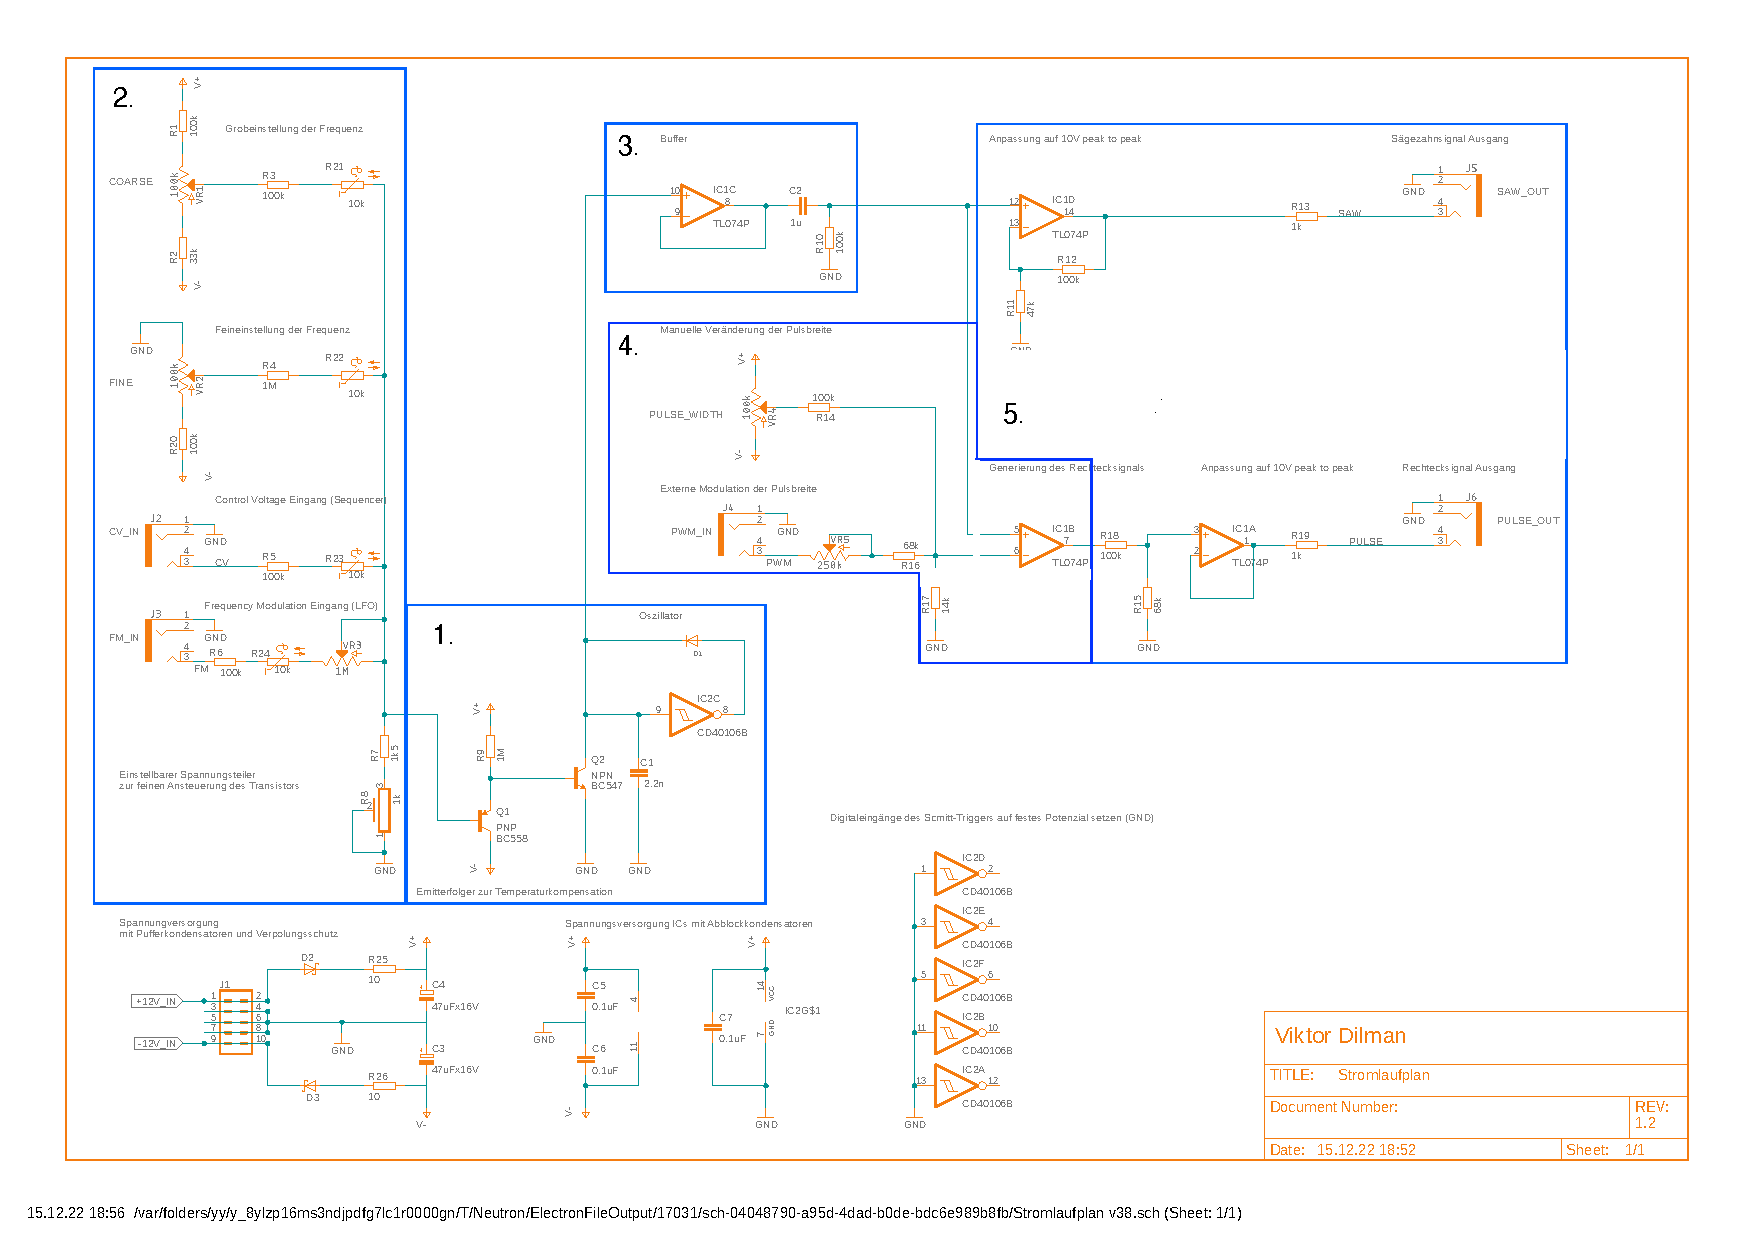
\includepdf[angle=270, clip, trim=1cm 0.8cm 0.8cm 0.8cm, scale=0.8] {figures/VCO_Stromlaufplan_v2_unterteilt.pdf}
%\caption{In Bereiche unterteilter Schaltplan des Sequenzers}
\caption{Schaltplan VCO}
\label{fig:VCO_Stromlaufplan}
\end{figure}

\newpage

\section{Platine}
Nachdem der Schaltplan in Fusion 360 erstellt und die Bauteile hinterlegt wurden, erfolgt die Erstellung des Platinenlayouts (siehe Abbildung \ref{fig:VCO Layout}).
Die äußeren Abmaße der Platine sind in Bezug auf die Höhe eines \textit{Euro Racks }von 128,5 mm beschränkt. 
Gewählt wurde eine Platinenhöhe von 100 mm, damit ausreichend Platz zur Befestigung der Leiterplatte gewährleistet ist.

\begin{figure}[h]
	\centering
	\setlength{\fboxsep}{1pt} %Abstand der Linien zur Abbildung
	\setlength{\fboxrule}{1pt} %Dicke der Linie
	\fbox{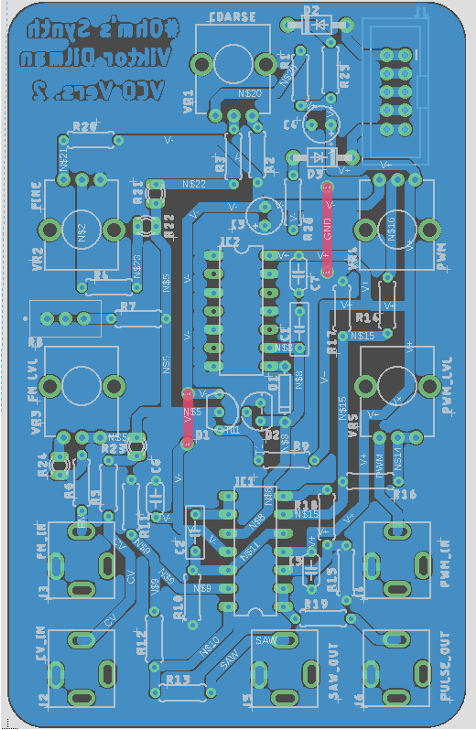
\includegraphics[width=0.5\textwidth]{figures/VCO_Layout}}
	\caption{VCO Layout in Fusion 360}
	\label{fig:VCO Layout}
\end{figure}

Die Bauteile wurden einerseits so positioniert, dass die Leiterbahnen möglichst kurz und überschneidungsfrei verlegt werden können.
Andererseits wurden die Potentiometer und Klinkenbuchsen logisch so angeordnet dass die zu einer Einbauklinkenbuchse gehörenden Potentiometer übereinander liegen.
Weiterhin wurde darauf geachtet, dass die Transistoren für die Temperaturkompensation möglichst nah aneinander positioniert werden.
Zudem sind die Stützkondensatoren der ICs möglichst nah an den Versorgungspins der Bauteile zu positionieren.

Bei der Erstellung der Platine wurde darauf geachtet möglichst eine Layer zu verwenden, um die Platine mit einer Platinenfräse herstellen zu können.
Dies ist von Vorteil, da bei der professionellen Anfertigung von Platinen von der Bestellung bis zur Lieferung einige Wochen vergehen können.
Ist der Zugang zu einer Fräse gegeben, kann die erstellte Platine sofort getestet und eventuelle Fehler ausgebessert werden.

Damit die Leiterplatte mit einer Platinenfräse angefertigt werden kann, ist eine relativ dicke Leiterbahnbreite erforderlich. 
Gewählt wurde deshalb eine Leiterbrahnbreite von 50 mil.
An den Stellen, an denen die Leiterbahnen nicht überschneidungsfrei verlegt werden konnten, wurden \textit{Vias} hinzugefügt und die Leiterbahn auf der anderen Seite fortgeführt.
Auf der gefrästen Platinen können diese \textit{Vias} mit Brücken verbunden werden.

Da für die verwendeten Einbauklinkenbuchsen keine passenden Bibliotheken existieren, mussten diese manuell anglegt werden.
Dafür wurde ein Symbol einer ähnlichen Klinkenbuchse verwendet und das Footprint nach dem Datenblatt des Herstellers erstellt wie in Abbildung \ref{fig:Klinkenbuchse Footprint} zu sehen.

\begin{figure}[h]
	\centering
	\setlength{\fboxsep}{1pt} %Abstand der Linien zur Abbildung
	\setlength{\fboxrule}{1pt} %Dicke der Linie
	\fbox{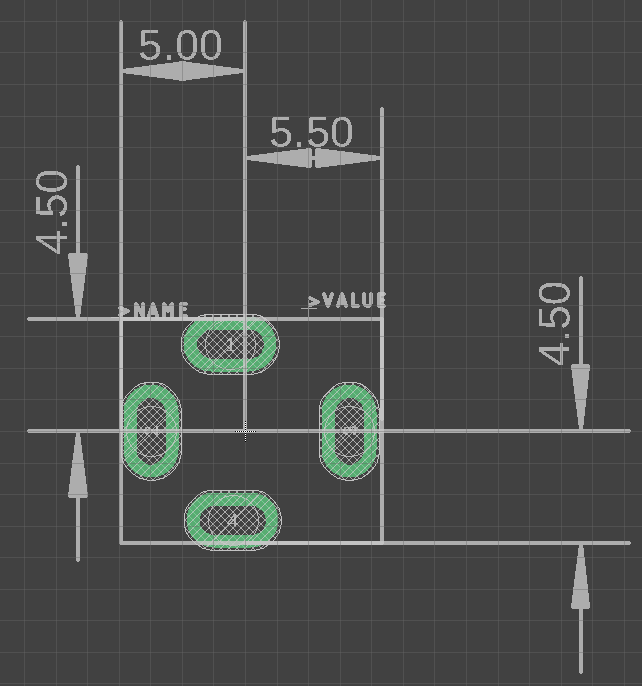
\includegraphics[width=0.3\textwidth]{figures/VCO_AUX_footprint}}
	\caption{Erstelltes Footprint der Einbauklinkenbuchse}
	\label{fig:Klinkenbuchse Footprint}
\end{figure}


Für das Fräsen der Platine wurden die Gerber-Files aus Fusion 360 exportiert.
%\begin{figure}[h]
%	\centering
%	\setlength{\fboxsep}{1pt} %Abstand der Linien zur Abbildung
%	\setlength{\fboxrule}{1pt} %Dicke der Linie
%	\fbox{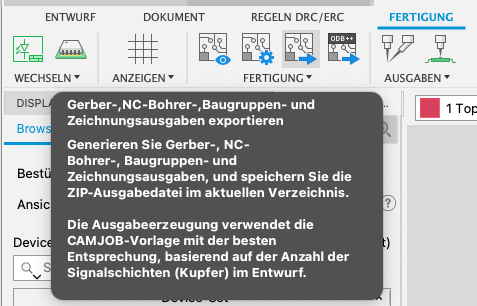
\includegraphics[width=0.5\textwidth]{figures/Fusion Export Gerber}}
%	\caption{Fusion 360 Gerber Export}
%	\label{fig:Gerber}
%\end{figure}
Die Leiterplatte wurde dabei mit einer Platinenfräse von \textit{Bantam Tools} hergestellt.
%\begin{figure}[h]
%	\centering
%	\setlength{\fboxsep}{1pt} %Abstand der Linien zur Abbildung
%	\setlength{\fboxrule}{1pt} %Dicke der Linie
%	\fbox{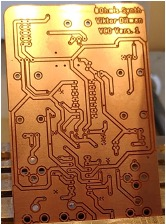
\includegraphics[width=0.5\textwidth]{figures/VCO_gefraest}}
%	\caption{VCO Platine gefräst}
%	\label{fig:VCO Fräse}
%\end{figure}
%\newpage
Nachdem die gefräste Platine getestet und validiert wurde, erfolgt die Bestellung der Leiterplatte beim Platinenhersteller \textit{Aisler}. 
In Abbildung \ref{fig:VCO_Front} ist die Vorderseite der Platine zu sehen.
Die Abbildung \ref{fig:VCO_Back} zeigt hingegen die Rückseite der VCO-Leiterplatte. 

\begin{figure}[h]
	\centering
	\begin{subfigure}{.5\textwidth}
		\centering
		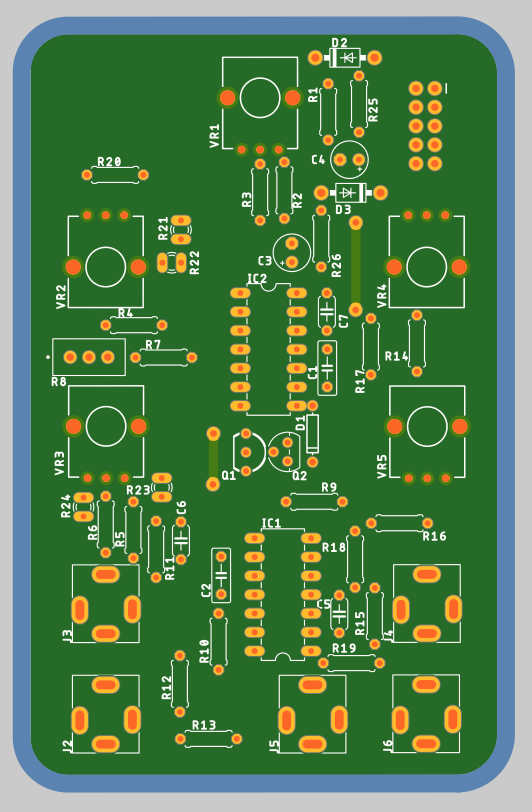
\includegraphics[width=0.75\textwidth]{figures/VCO_Rendering_Front}
		\caption{Vorderseite}
		\label{fig:VCO_Front}
	\end{subfigure}%
	\begin{subfigure}{.5\textwidth}
		\centering
		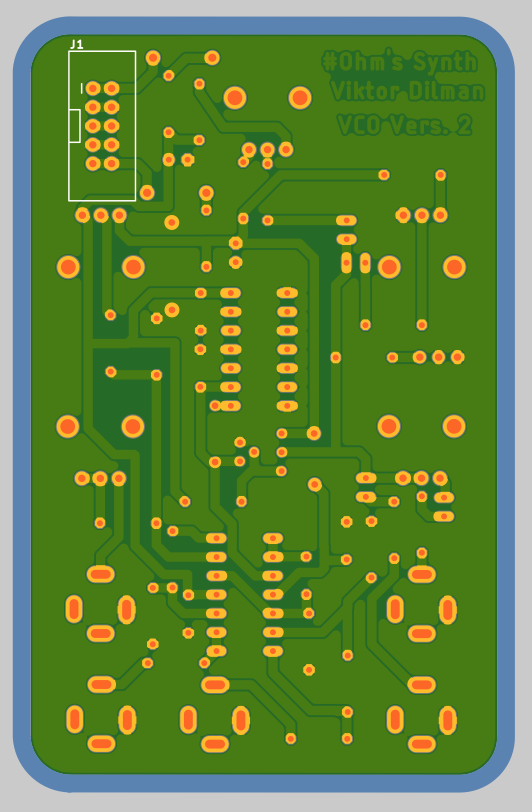
\includegraphics[width=0.75\textwidth]{figures/VCO_Rendering_Back}
		\caption{Rückseite}
		\label{fig:VCO_Back}
	\end{subfigure}
	\caption{VCO Leiterplatte}
	\label{fig:VCO Leiterplatte}
\end{figure}


\newpage
\section{Mechanischer Aufbau}
Mithilfe der \textit{Fusion 360}-Funktionalität der Übertragung einer 2D- auf eine 3D-Leiterplatte wurde eine Abdeckung konstruiert (siehe Abbildung \ref{fig:VCO Frontplattemit 3D-Leiterplatte}).
Dies hat den Vorteil, dass für die Potentiometer und Klinkenbuchsen die Aussparungen an der Frontplatte exakt positioniert werden konnten.
Die Abdeckplatte wird mithilfe der Gewindeschrauben der Einbauklinkenbuchse an die Platine befestigt.
Zusätzlich werden auf die Potentiometer Abdeckkappen angebracht, die zusätzlichen Halt bieten.
An den Ecken der Frontplatte werden Aussparungen vorhergesehen, um das Modul in einem Eurorack-Gehäuse befestigen zu können.
Schließlich wurde die Frontplatte aus Plexiglas mit einem Laser-Cutter gefertigt.

\begin{figure}[h]
	\centering
	\setlength{\fboxsep}{1pt} %Abstand der Linien zur Abbildung
	\setlength{\fboxrule}{1pt} %Dicke der Linie
	\fbox{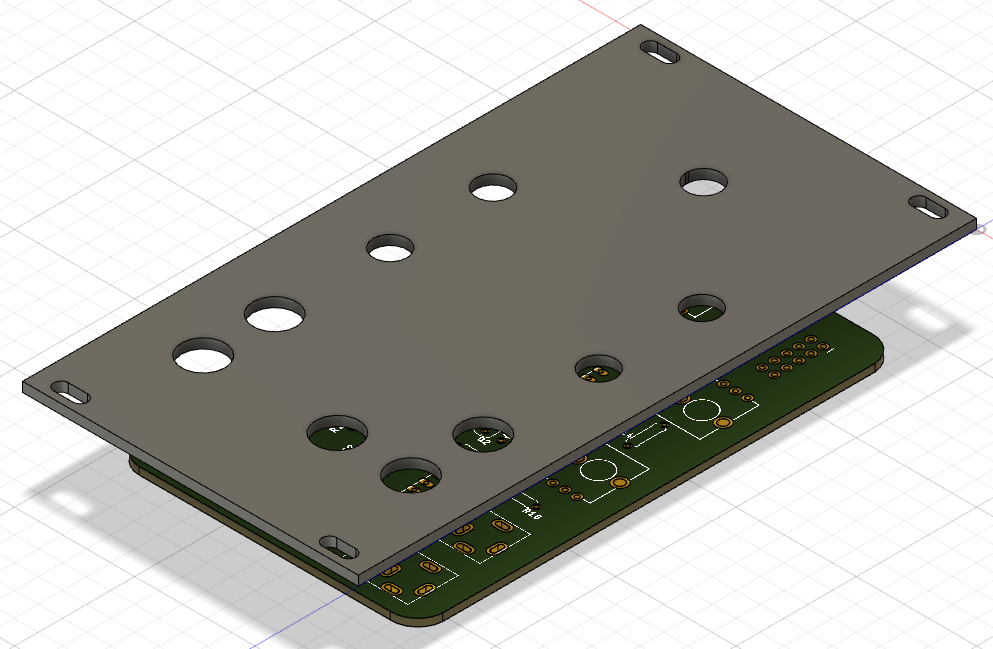
\includegraphics[width=0.8\textwidth]{figures/VCO_Frontplatte_schraeg}}
	\caption{VCO Frontplatte}
	\label{fig:VCO Frontplattemit 3D-Leiterplatte}
\end{figure}
\chapter{Sequenzer}
\label{ch:Sequenzer}
\section{Allgemeines}
Bei dieser Umsetzung eines Sequenzers wurde sich für maximal fünf alternierende Spannungspegel entschieden. In der Literatur ist diese Unterart als 5-Step-Sequencer bekannt, welche wegen ihrer markanten Charakteristik zum Beispiel im bekannten >>Hier Name des Syntis im Labor einsetzten<< Synthesizer eingesetzt wird. >>Als Quelle Manual von genanntem Synti nennen<<. Über zwei in der Handebene verbaute Kippschalter kann alternativ zwischen 3- bzw. 4-Stufen-Betrieb gewählt werden. Welcher Schritt aktuell aktiv ist wird durch Status-LEDs in der Frontplatte angezeigt.\\
Als Spannungsversorgung erhält der Sequenzer \textpm 12 Volt durch das verbaute Netzteil (vgl. Kapitel \ref{ch:Netzteil}). Optional kann ein externes Clock-Signal, beispielsweise von einem LFO (vgl. Kapitel \ref{ch:LFO}), angeschlossen werden. Der eigene Takt wird dadurch überbrückt, wodurch das Modul flexibel eingesetzt werden kann. Des Weiteren kann die Sequenz durch ein externes Signal zurückgesetzt werden. Dadurch wird automatisch wieder bei der ersten Stufe der Sequenz begonnen, wodurch dem Nutzer weiterer musikalischer Freiraum freigeräumt wird.\\
Das Sequenzer-Modul verfügt über drei abgreifbare Ausgangssignale. Ein Clock-Signal, welches über ein Potentiometer in der Handebene parametrisiert werden kann, gibt den internen Takt des Moduls vor, und kann von außerhalb abgegriffen werden. Dessen Spannung toggelt dabei zwischen -12 und +12 Volt. Die Control Voltage (CV) wird zumeist dem VCO (vgl. Kapitel \ref{ch:VCO}) zur weiteren Verarbeitung überreicht. Dabei handelt es sich um eine alternierende Spannungsfolge, welche zwischen 0 und 5 Volt schwanken kann. Die einzelnen Spannungspegel der bis zu fünf Stufen werden durch ein jeweiliges Potentiometer in der Handebene eingestellt. Das dritte Ausgangssignal des Sequenzers bildet der Gate. Ähnlich dem CV wird eine alternierende Spannungsfolge von bis zu fünf Stufen ausgegeben, wobei eine Stufe in zwei Abschnitte geteilt wird. Der erste Abschnitt beträgt, abhängig dem jeweiligen Kippschalter in der Handebene, entweder +12 oder 0 Volt. Der zweite Abschnitt führt immer 0 Volt. Der Gate verhält sich somit ähnlich dem Clock-Signal. Er führt jedoch niemals eine Negative Spannung und seine Stufen sind manuell zuschaltbar. In der Regel wird der Gate als Eingangssignal für den ADSR hergenommen.

\section{Schaltplan}
\newpage	%Seite leer beenden und Umbruch

\begin{figure}[h]
	\centering
	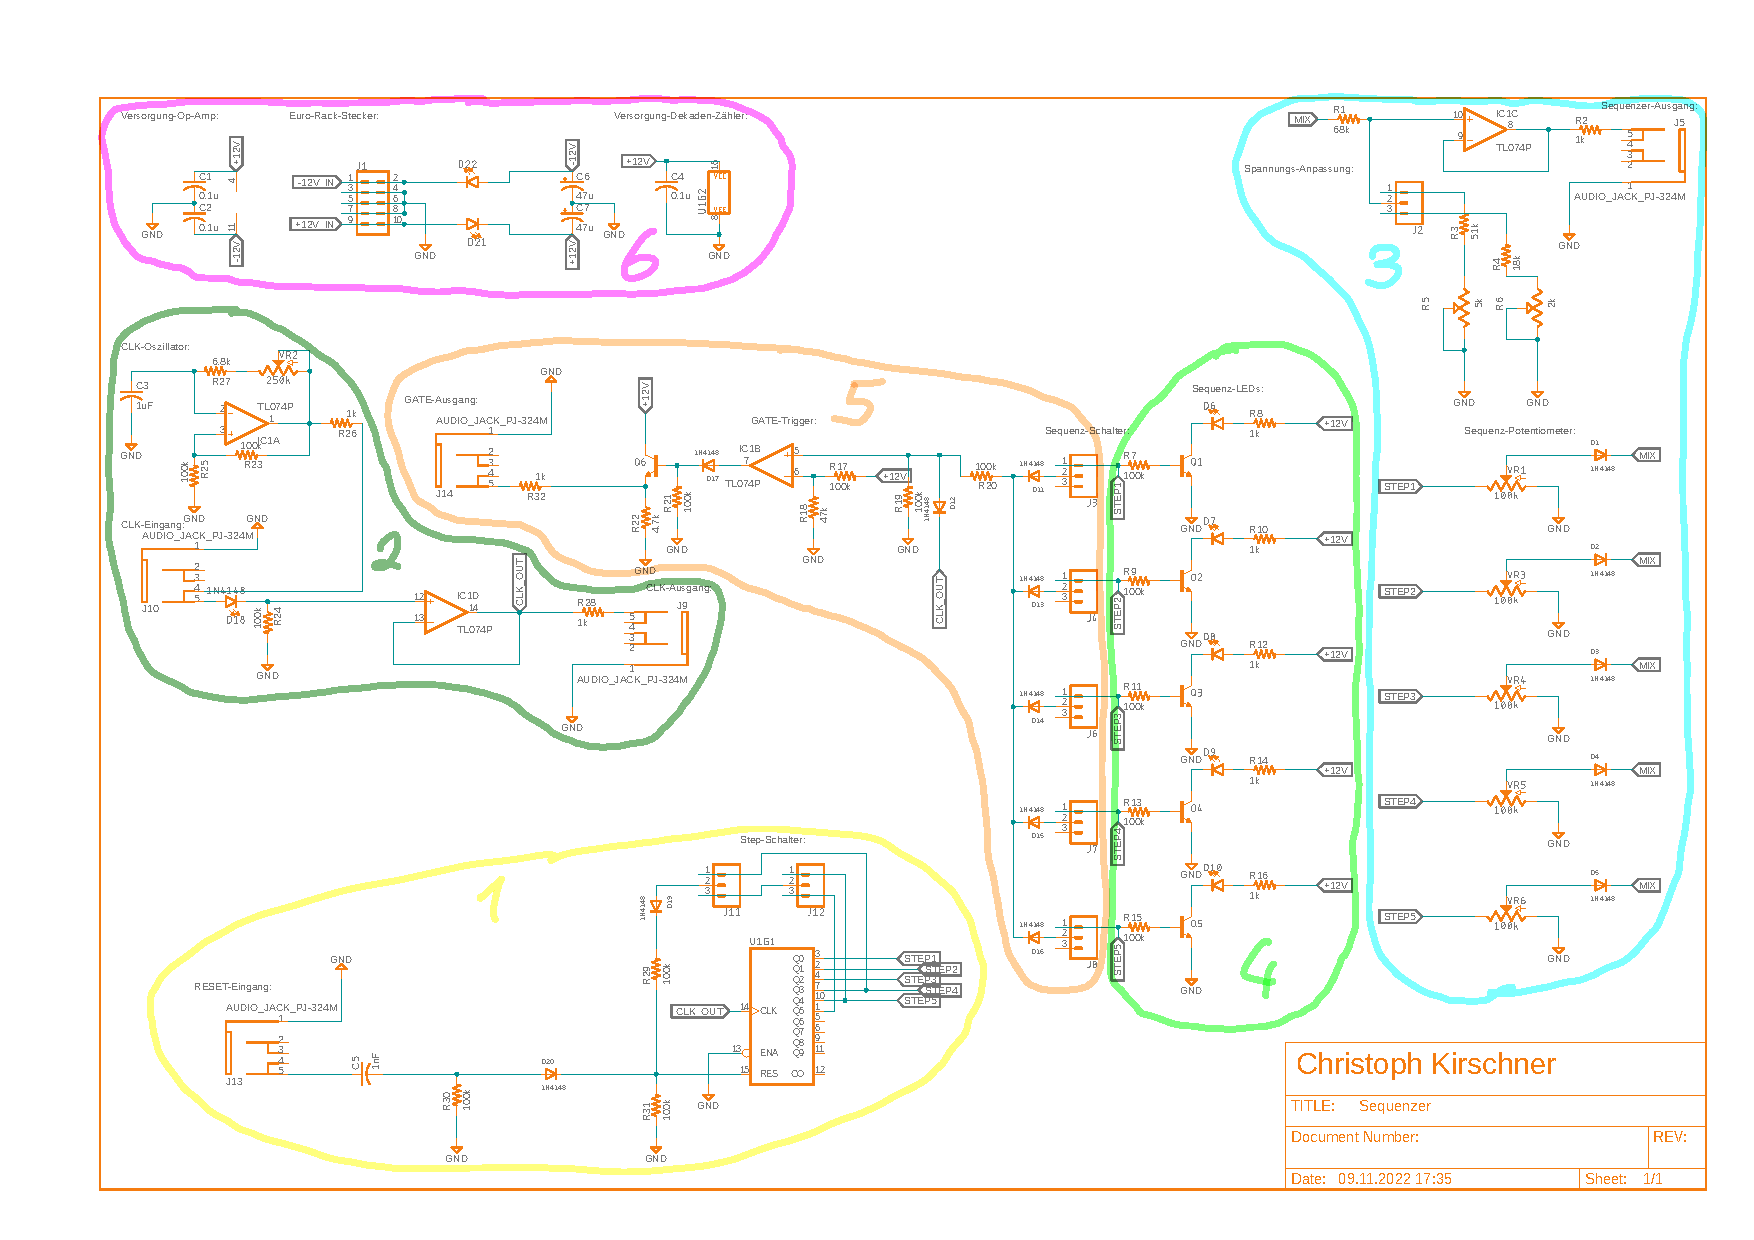
\includepdf[angle=270, clip, trim=1.7cm 0.85cm 0.8cm 1.65cm, scale=0.8] {figures/Schaltplan_Sequenzer_Christoph_Kirschner_unterteilt.pdf}
	\caption{Schaltplan der Sequenzer-Platine}
	\label{fig:Schaltplan_des_Sequenzers}
\end{figure}

\newpage	%Seite leer beenden und Umbruch
Der Schaltplan des Sequenzers lässt sich, wie in Abbildung \ref{fig:Schaltplan_des_Sequenzers} gezeigt, in sechs Bereiche unterteilen. Der Bereich eins ist zuständig für das Durchschalten der Zustände.
Die wesentliche Komponente ist dabei das Bauteil U1G1. Es handelt sich dabei um einen CD4017 Dekadenzähler, der durch das Toggeln des Clock-Signals die verschiedenen Zustände durchschaltet. Der Sequenzer ist für eine Sequenz von maximal 5 Stufen ausgelegt. Durch die beiden Schalter J11 und J12 kann diese jedoch auf 4 bzw. 3 Stufen reduziert werden, was sich an der Rückführung der jeweiligen Stufen auf den RESET-Pin erkennen lässt. Durch den RESET-Eingang J13 lässt sich zusätzlich ein externes Signal einbinden, was einen Fremd-RESET ermöglicht.\\
Der zweite Bereich des Schaltplans kümmert sich um das Clock-Signal. Dafür wird der Operationsverstärker (OPV) IC1A sowohl über eine Mitkopplung durch R23, als auch über eine Gegenkopplung durch R27 und VR2 betrieben. Der dadurch realisierte Negativ-Impedanz-Konverter läd bzw. entläd den Kondensator C3 in Abhängigkeit des Potentiometers VR2. Das daraus entstehende Clock-Signal wird über einen Buffer (IC1D) geführt und unter anderem über den Klinkenausgang J9 nach außen zur Verfügung gestellt. Der Klinkeneingang J10 ist zusätzlich in der Lage das interne Clock-Signal durch ein extern angelegtes zu übersteuern.\\
Im dritten Abschnitt werden den verschieden Zuständen ihre jeweiligen Spannungen zugewiesen. Um das zu erreichen wird jedes Zustandssignal über ein separates Potentiometer gegen Masse geführt. Der Abgriff wird anschließend durch jeweilige Dioden vor rückfließenden Strömen geschützt und zusammengeführt. Um das Spannungssignal nun zu limitieren, wurden zwei Spannungsteiler R1 und R3 für 0 - 5 Volt sowie R1 und R4 für 0 - 2.5 Volt eingesetzt. Um Bauteiltoleranzen kompensieren zu können wurden zusätzlich zwei Trimmer R5 und R6 verbaut. Zwischen den Spannungsbereichen kann über den Schalter J2 gewechselt werden (default: 0 - 5 Volt). Danach kommt wieder ein Buffer (IC1C) und in Reihe dazu der Widerstand R2. Dieser Widerstand sorgt dafür, dass im Falle eines Kurzschlusses der Fehlerstrom begrenzt und dadurch kein Schaden in der Schaltung entsteht. Der so entstandene CV kann über den Klinkenausgang J5 abgegriffen werden.\\
Der vierte Bereich des Schaltplans (vgl. Abbildung \ref{fig:Schaltplan_des_Sequenzers}) ermöglicht das Ablesen des aktiven Zustandes über die Frontplatte. 
Dafür wird für jeden möglichen Zustand eine LED (D6 - D10) angeschaltet, welche nach außen geführt ist. 
Die LEDs werden durch eine Emitterschaltung eines 2N3904 NPN Transistor angesteuert. Somit werden die Spannungssignale entlastet und möglichem Schaden vorgebeugt.\\
Die Funktionalität des Gate-Ausgangs wird in Bereich fünf umgesetzt. Die verschiedenen Stufenspannungen des Dekadenzählers aus Bereich eins werden jeweils über einen Kippschalter sowie eine Diode geführt und danach vereint. Die Schalter ermöglichen ein manuelles Zu- bzw. Wegschalten der einzelnen Stufe im resultierenden Gate-Signal. Die Dioden verhindern, wie auch bei der Umsetzung des CV, ein rückfließen der Ströme in die anderen Stufensignale. Nach der Zusammenführung der Signale folgt der Widerstand R20, sowie das über eine Diode begrenzte Clock-Signal. Das Clock-Signal sorgt dafür das der Gate in jedem Zyklus für die halbe Zeit auf 0 Volt gesetzt wird. Durch den Widerstand R20 wird einem Kurzschluss in diesem Pfad vorgebeugt. Der Widerstand R19 verhindert einen undefinierten Zustand sobald ein Stufe durch einen Kippschalter weggeschaltet wird. Allerdings bilden R19 und R20 einen ungewollten Spannungsteiler, der aus den gewünschten +12 Volt +6 Volt macht. Aus diesem Grund wurde ein weiterer OPV als einfacher Komparator verbaut. Die Widerstände R17 und R18 sorgen für eine Vergleichsspannung von 3.8 Volt am nicht-invertierenden Eingang, weshalb bei den anliegenden +6 Volt problemlos durchgeschaltet wird. Der negative Teil der Spannung wird anschließend durch die Diode D17 sowie den Pulldown-Widerstand R21 unterbunden. Um der resultierenden hohen Impedanz sowie der begrenzt möglichen Stromentnahme der aktuellen Schaltung entgegenzuwirken, wurde der Ausgang mit einem BC547 NPN Transistor versehen. Dieser wurde als Kollektorschaltung implementiert sowie, um Kurzschlüsse zu vermeiden, mit einem weiteren Widerstand R32 verbaut. Der Gate kann somit über den Klinkenausgang J14 von außen abgegriffen werden.\\
Der letzte Bereich ist zuständig für die Spannungsversorgung des gesamten Moduls. Das Netzteil (vgl. Kapitel \ref{ch:Netzteil}) versorgt den Sequenzer mit \textpm 12 Volt durch den Euro-Rack-Stecker. Um Verpolung vorzubeugen, wurden zwei Dioden D21 und D22 verbaut. Anschließend werden die beiden Spannungen mit den Kondensatoren C6 und C7 gegen Masse gepuffert. Weitere Pufferkondensatoren wurden in der Versorgung der OPV als auch in der Versorgung des Dekadenzählers vorgesehen \cite{seq_manual}.

\section{Platine}
\begin{figure}[h]
	\centering
	\setlength{\fboxsep}{1pt} %Abstand der Linien zur Abbildung
	\setlength{\fboxrule}{1pt} %Dicke der Linie
	\fbox{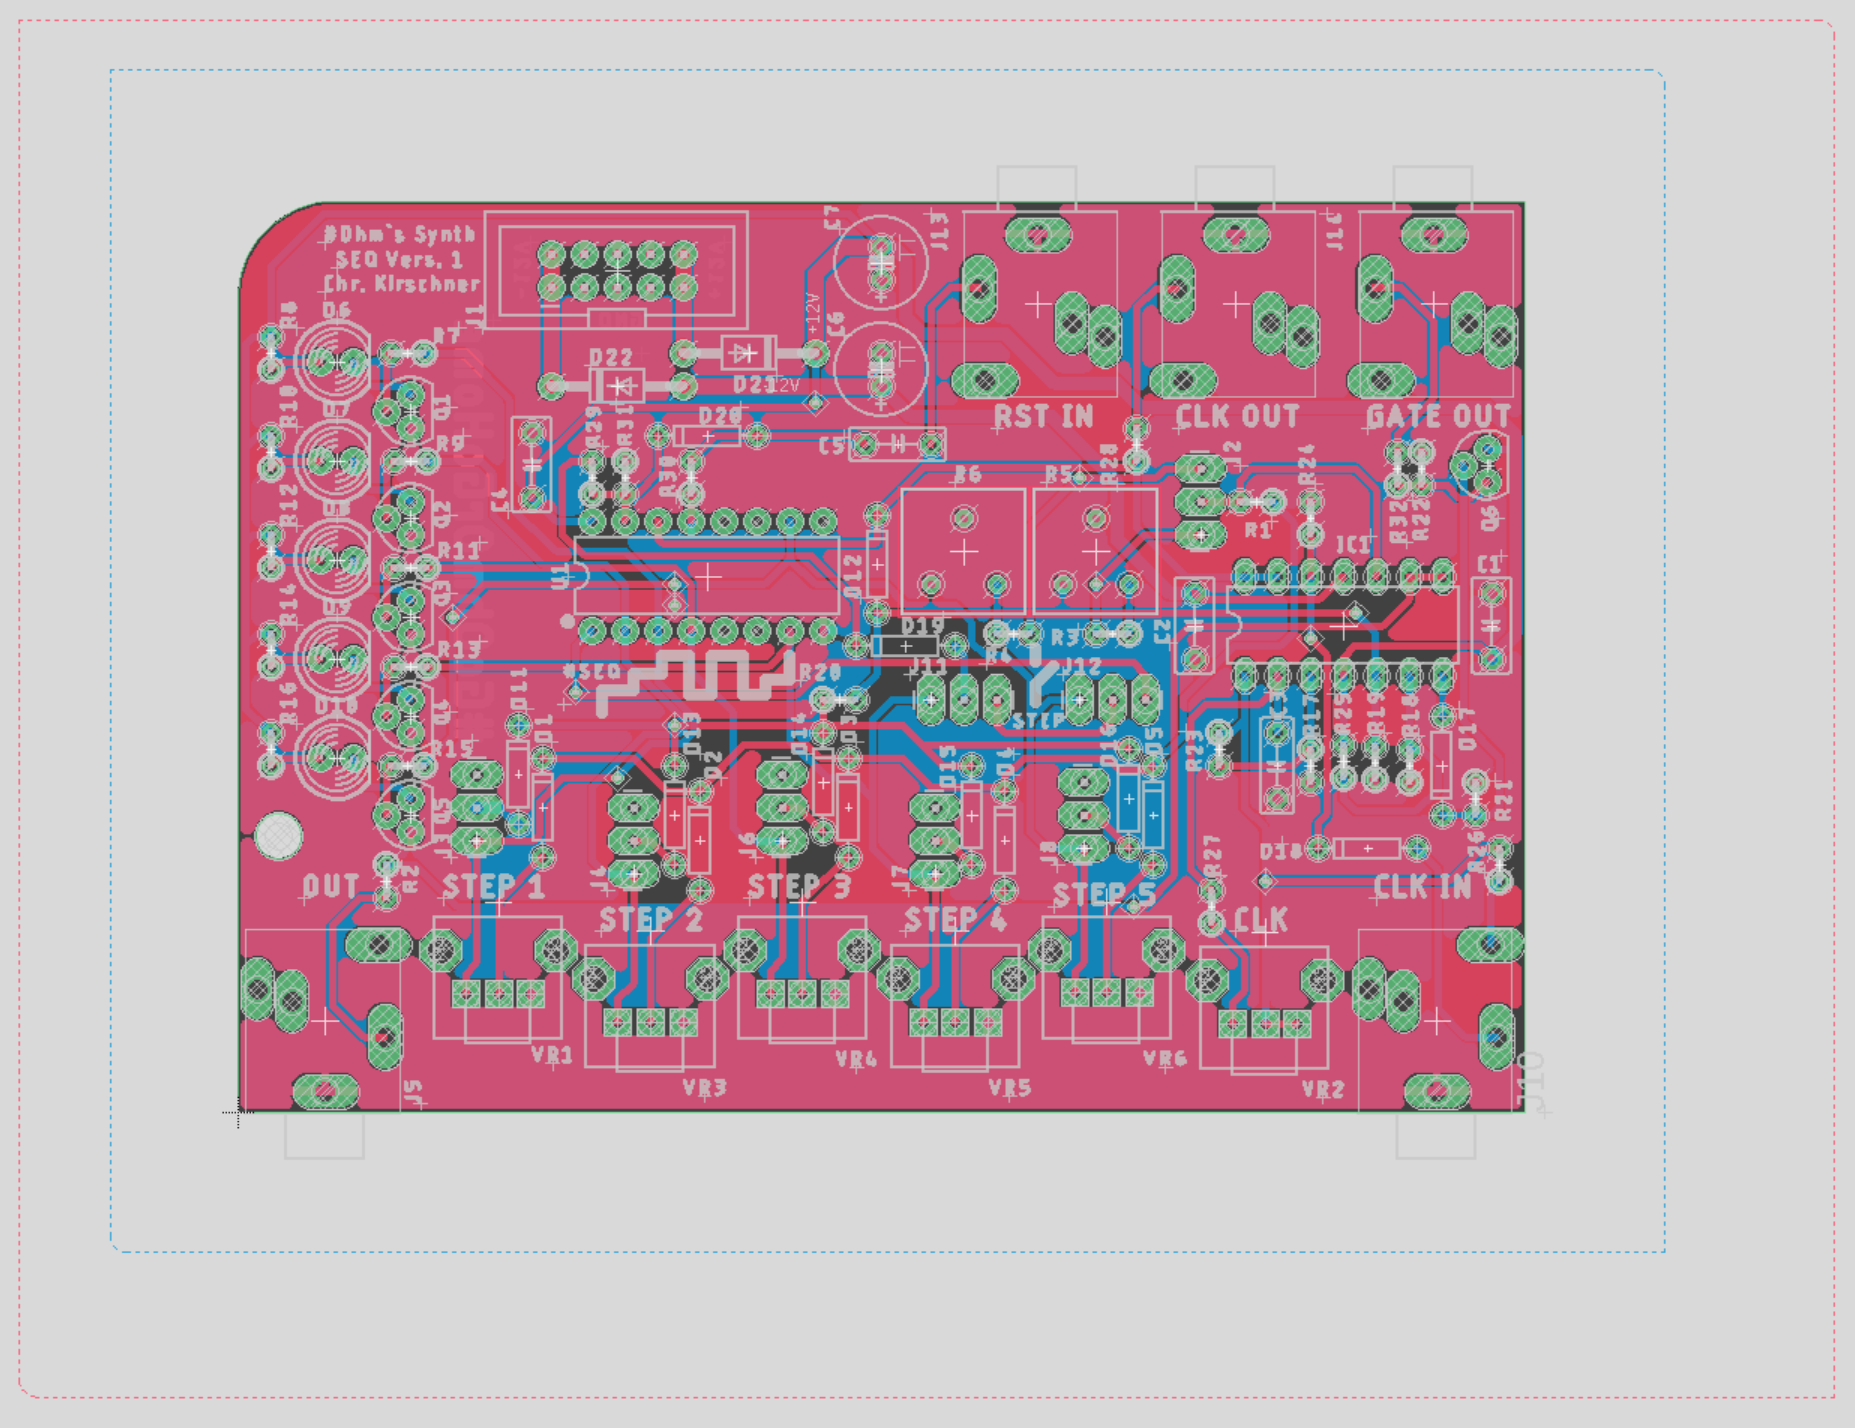
\includegraphics[width=1\textwidth]{figures/Sequenzer_Layout.PNG}}
	\caption{Ausschnitt des SEQ-Platinen-Layouts aus Fusion360}
	\label{fig:PCB_SEQ}
\end{figure}
\FloatBarrier
 
\section{Mechanischer Aufbau}

\chapter{Filter}
\label{ch:concept}
\section{Allgemeines}


\section{Schaltplan}
bla bla bla

\section{Platine}
bla bla bla

\section{Mechanischer Aufbau}
bla bla bla
\chapter{Mischer}
\label{ch:concept}
\section{Allgemeines}
Der Audio Mixer verknüpft verschiedene, von den anderen Bauteilen des modularen Synthesizers erzeugte Eingangssignale (Klangquellen) miteinander. Das heißt er mischt, kombiniert und gleicht verschiedene Klänge und Audiosignale aus, wodurch neue Signalformen
und Klänge generiert werden können. Die entstehenden kombinierten Signale werden an den Filter weitergeleitet.


\section{Schaltplan}
Dieser Abschnitt beschreibt den Schaltplan des Mischers in Abbildung \ref{fig:schaltplan_mixer}. 
Dazu werden die einzelnen Teilbereiche des Schaltplans vorgestellt.

IN1-IN3 sind die Audioeingangsbuchsen, INV OUT-CLIP OUT sind die Audio-Ausgangsbuchsen.

Der Teilbereich 1 des Schaltplans ermöglicht die Anpassung der Lautstärke der Signale in jedem Bereich zwischen 0\% und 100\%. 
Ein zentrales Bauteil ist der Vierfach-Operationsverstärker TL074P. Die drei verbauten Potentiometer regeln die Levels der Eingangssignale.

Der zweite Teilbereich lässt eine Modulation des Ausgangssignals (hinsichtlich Verzerrung und Wärme des Klangs) zu. Der Strom fließt durch die Diode nur in eine Richtung. Der 100k-Widerstand wird benötigt, um die Gefahr eines Kurzschlusses zu beheben. Denn ohne diesen Widerstand würde der Strom exponentiell steigen, da sich die Diode unbegrenzt öffnet, wenn die Spannung ansteigt. Die Spannung über der Diode bleibt konstant, wenn der Operationsverstärker einen bestimmten Threshold übersteigt. Dieser Effekt nennt sich Soft Clipping. Die zweite verbaute Diode erfüllt einen entsprechenden Zweck für negative Spannung. 
In Teilbereich 3 ist XP1 ein Standard-Eurorack-Stromanschluss. Es handelt sich um eine 2x5-Stiftleiste mit einem Schlüssel, die eine versehentliche Stromversorgung mit umgekehrter Polarität verhindern soll, denn ein falscher Anschluss der Stromversorgung würde zu dauerhaften Schäden am Modul führen. D3 und D4 sind Schottky-Dioden, die die Stromversorgung mit umgekehrter Polarität doppelt sichern.
Auf den + und -12-V-Schienen wurden zwei 10-Ohm-Widerstände (R15 und R16) mit Entkopplung verwendet und Kondensatoren C1 - C4. In Kombination mit R15 und R16 kompensiert C1 und C2 Niederfrequenzschwankungen, während C3 und C4 Funkfrequenzen, Hochfrequenzspitzen von Schaltnetzteilen und schnelle, von anderen Modulen erstellte Spitzen herausfiltern.
Die Kondensatoren C5 - C8 sind zusätzliche Entkopplungskondensatoren.

\begin{figure}[h]
	\centering
	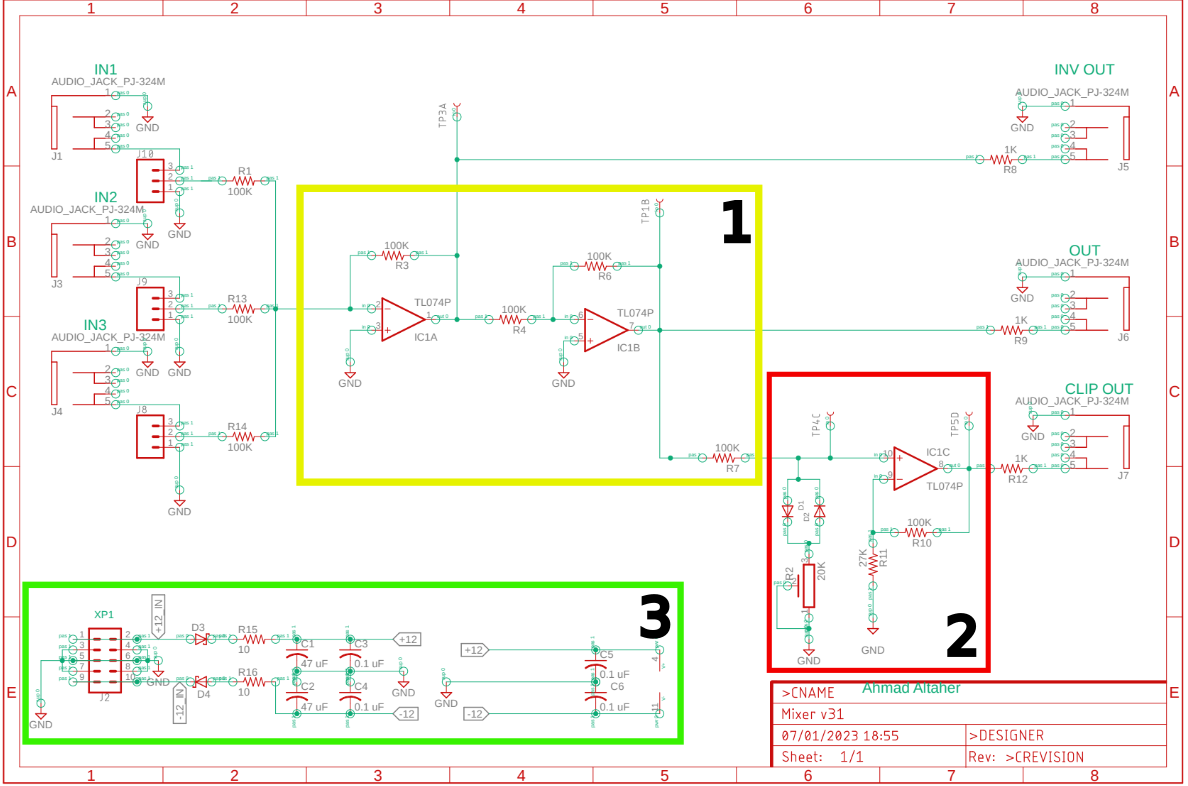
\includegraphics[angle=270, width=1\textwidth]{figures/SchaltplanMixer_new.png}
	\caption{Ausschnitt des Mischer-Schaltplanes aus Fusion360 \cite{mixer_manual}}
	\label{fig:schaltplan_mixer}
\end{figure}
\FloatBarrier

\section{Platine}
\begin{figure}[h]
	\centering
	\setlength{\fboxsep}{1pt} %Abstand der Linien zur Abbildung
	\setlength{\fboxrule}{1pt} %Dicke der Linie
	\fbox{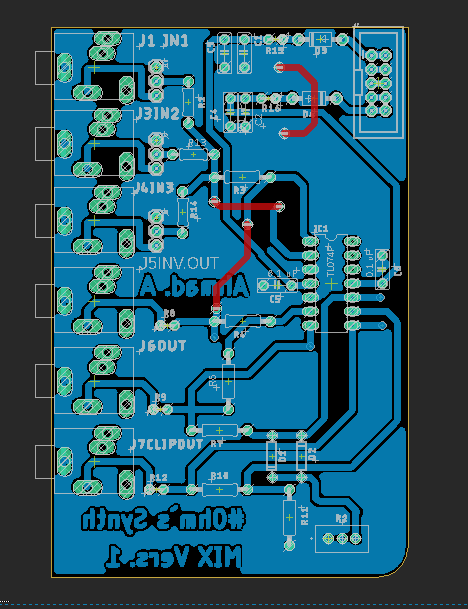
\includegraphics[width=0.7\textwidth]{figures/mixer_platine.png}}
	\caption{Ausschnitt des Mischer-Platinen-Layouts aus Fusion360 (Unterseite)}
	\label{fig:platine_mixer}
\end{figure}
\FloatBarrier
\chapter{Gehauese}
\label{ch:concept}
\section{Allgemeines}
bla bla bla

\section{Mechanischer Aufbau}
bla bla bla
\chapter{Fazit}\label{ch:fazit}
Ziel des Projekts war die Entwicklung eines modular aufgebauten analogen Synthesizer zur elektronischen Klangsynthese.
Im Zuge des Projekts sollten Fertigkeiten bezüglich Konzeption, Entwurf und Fertigung von analogen Schaltungen.
Es wurde von jedem Teammitglied der komplette Prozess von Konzeption der Schaltung, Simulation der Eigenschaften, Layout einer Leiterplatte und deren Bestückung sowie das Design einer Frontplatte durchlaufen. Somit kann der Gewinn bzw. die Weiterentwicklung dieser spezifischen Fertigkeiten als voller Erfolg angesehen werden. Dass grundsätzlich alle Module bis auf einzelne kleine Mängel funktionieren spricht auch für den Erfolg des Projekts.\\
Es konnten bis auf den ADSR und den VCA alle Module realisiert werden. Das liegt an der im Vorfeld etwas unterschätzten Erwartungshaltung bezüglich des Aufwands der tatsächlichen Realisierung inkl. Bestückung und Debugging.  
Das ist aber aus Sicht des Teams in Ordnung, da der Großteil der Gruppe noch nie solche Tätigkeiten gemacht hatte.
Neben dem Gewinn an neuen Fertigkeiten war vor allem der Spaß am Entwicklen ein immer präsenter Gast in den Laborterminen.
Abschließend bedanken wir und bei Herrn Zimmermann für das schnelle und zuverlässige Abwickeln der Bauteil-Bestellungen und die Betreuung im Labor und bei Herrn von Hoffmann für die gute Zusammenarbeit.



% remove if not needed
\appendix
%\chapter{Supplemental Information}\label{app:supplemental-information}

\Blindtext



\backmatter

\lstlistoflistings
\cleardoublepage

\printbibliography

\end{document}
